\Titre{CIA: Confidentiality, Integrity, Availability}

\begin{document}

\begin{reveals}
                
\maketitle




\section{Base Concepts}

\subsection{Security Properties}

\begin{frame}[c]{}
  
  \begin{block}{Definition (NIST)}
    \textcolor{red}{\bf Information Security:} The protection of
    information and information systems from unauthorized access, use,
    disclosure, disruption, modification, or destruction in order to
    provide \textbf{confidentiality}, \textbf{integrity}, and
    \textbf{availability}.
  \end{block}
\end{frame}

\begin{frame}[c]{Confidentiality (1/2)}
  
  \begin{block}{Data Confidentiality}
    Preserving authorized restrictions on information access and
    disclosure, including means for protecting personal privacy and
    proprietary information
  \end{block}

  \vfill

  \begin{block}{Exemples}
    \begin{itemize}
    \item Secret informations
    \item Know-how in a company
    \item Strategy
    \end{itemize}
  \end{block}
\end{frame}

\begin{frame}[c]{Confidentiality (2/2)}
  
  \begin{block}{Privacy}
    Assurance that the confidentiality of, and access to, certain
    information about an entity is protected
  \end{block}

  \vfill

  \begin{block}{Examples}
    \begin{itemize}
    \item Individual Preferences
    \item Right-to-be-forgotten
    \item Entails some organisational and cross-organisational access control
    \end{itemize}
  \end{block}
\end{frame}


\begin{frame}[c]{Integrity (1/2)}
  
  \begin{block}{Data Integrity}
    Guarding against improper information modification or destruction,
    and includes ensuring information \textbf{non-repudiation} and
    \textbf{authenticity}.
  \end{block}

  \vfill

  \begin{block}{Examples}
    \begin{itemize}
    \item Trust in data (fake polls, fake news)
    \item Trust in the process producing data (steal the vote)
    \end{itemize}
  \end{block}

\end{frame}

\begin{frame}[c]{Integrity (2/2)}
  
  \begin{block}{System Integrity} 
    the quality of an IT system that reflects the logical correctness
    and reliability of the operating system; the logical completeness
    of the hardware and software that implements the protection
    mechanisms; and the consistency of the data structures and
    occurrence of the stored data.
  \end{block}

  \vfill

  \begin{block}{Examples}
    \begin{itemize}
    \item No malwares nor viruses
    \item No illegal softwares
    \end{itemize}
  \end{block}

\end{frame}

\begin{frame}[c]{Availability}
  
  \begin{block}{Definition}
    Ensuring timely and reliable access to and use of information.
  \end{block}

  \vfill

  \begin{block}{Examples}
    \begin{itemize}
    \item A slow web site
    \item No ransomware
    \end{itemize}
  \end{block}

\end{frame}

\begin{frame}[c]{Authenticity}
  
  \begin{block}{Definition}
    \begin{itemize}
    \item For an asset, integrity and proof of origins and integrity
      of the process that created that asset
    \item For a person, a proof of the identity of that person 
    \end{itemize}
  \end{block}

  \vfill

  \begin{block}{Examples}
    \begin{itemize}
    \item Sotware traceability, including during development
    \item Trust in a web site
    \end{itemize}
  \end{block}
\end{frame}


\begin{frame}[c]{Auditability}
  
  \begin{block}{Definition}
    the proper association of each operation of a system with a person
    responsible for that operation
  \end{block}

\end{frame}


\section{Challenges in Information Security}

\begin{frame}[c]{Understanding the Properties}
  
  \begin{block}{Simple sounding properties}
    \begin{itemize}
    \item A security goal is usually expressible in a few words
    \item The exact meaning however is often elusive
    \end{itemize}
  \end{block}

  \vfill

  \begin{block}{Example: a vote must be kept secret}
    \only<2->{
      \begin{itemize}
      \item If everyone votes for the same outcome, everyone knows
        what everyone has voted for (it's independent of the system
        employed to vote)
      % exemple: Beyoncé vient faire un concert spécial pour vous la semaine prochaine
        \only<3->{\item In real elections, there is only a few
          outcomes possibles, but there is a huge number of passwords,
          and they can also in principle all be written. So what does
          it mean when you say you know something? You can write it
          always/with a positive probability of success/sometimes ?}
    % exemple: voulez-vous que Sarkozy vienne faire un discours, 3 possibilités,
    % oui, non, ne vote pas
        \only<4->{\item Process integrity: is it really the vote a
          person wanted to cast, or was s/he coerced into casting it?
          Is it possible that you have no choice on the possible
          available candidates, so the vote you cast is meaningless?}
    \end{itemize}}
  \end{block}

\end{frame}

\begin{frame}[c]{Security is not Safety}
  
  \begin{block}{Safety}
    \begin{itemize}
    \item A system is known
    \item The environment is modeled with probabilities of bad things happening
    \item We want safety wrt these probabilities
    \end{itemize}
  \end{block}

  \vfill

  \begin{block}{Security}
    \begin{itemize}
    \item The execution environment knows what he does (is an
      \emph{attacker}), and he wants you to fail
    \item Security is parameterised by the computing capabilities of
      the attacker
      \begin{itemize}
      \item quantum cryptography
      \item \url{https://threatpost.com/pita-side-channel-attack-steals-gpg-key-from-laptops/113447/}
      \end{itemize}
    \item The most common security flaws come from highly improbable
      corner cases (is there someone with a name of more than 200 characters?)
    \end{itemize}
  \end{block}

\end{frame}

\begin{frame}{Hard Problems}

    \begin{block}{Need to be resilient against unforeseen threats}
    \begin{itemize}
    \item Security building blocks are \emph{hard}
    \item Often very abstract \textit{wrt} the simple property you
      want
    \end{itemize}
  \end{block}

  \vfill

  \begin{block}{Example}
    Cryptography: Mathematics on very abstract objects. 
      \begin{center}
        A sobering read: Weil Pairing (or lattices) for asymmetric
        cryptography
      \end{center}
  \end{block}


\end{frame}

\begin{frame}[c]{Intricate Mechanisms}
  
  \begin{block}{Note}
    \begin{itemize}
    \item hard: need full-time study or a PhD in the field to
      understand what really happens
    \item intricate: need to spend a lot of times to gather lot of
      different but simple pieces
    \end{itemize}
  \end{block}

  \vfill

  \begin{block}{Partial Information}
    \begin{itemize}
    \item Always need to reason by alternating different point of
      view, with different information
    \item Information diffusion and its consequences is hard to understand
    \item Example: social engineering, exploitation of publicly
      available data by hackers, information escalation
    \end{itemize}
  \end{block}

  \vfill

  \begin{block}{Distributed Systems}
    \begin{itemize}
    \item Security \emph{protocols} are employed to diffuse information in a system
    \item Harder than regular communication protocols since
      participants may not want to collaborate
    \end{itemize}
  \end{block}

\end{frame}

\begin{frame}[c]{Security Arms race}
  
  \begin{block}{Consequence of the preceding slides}
    \begin{itemize}
    \item Impossible (in practice) to predict all the consequences of a security mechanism
    \item By necessity, the defender has to protect assets against \emph{known} attacks
    \item The attacker tries to innovate and implement new attacks
      (\emph{e.g.} by discovering new vulnerabilities)
      %exemple: fichier de mots de passe
    \end{itemize}
  \end{block}

\end{frame}

\begin{frame}[c]{Handicaps for a Secure Architecture (1/2)}
  
  \begin{block}{Financial Handicap}
    \begin{itemize}
    \item Hard to quantify RoI: cost of analysis, cost of problem
      resolution, cost of vulnerability exploitation, probability of
      exploitation
    \item Lot of memes: security engineer getting a hard treatment for
      not implementing a solution he proposed earlier, but was refused
    \end{itemize}
  \end{block}

  \pause\vfill

  \begin{block}{Moving Landscape}
    \begin{itemize}
    \item Software have new versions, bugs are discovered and corrected regularly
    \item A complete infrastructure (CVE, CVM, etc.) and tools are
      dedicated just to get an up-to-date picture of a system
    \end{itemize}
  \end{block}

\end{frame}

\begin{frame}[c]{Handicaps for a Secure Architecture (2/2)}

  \begin{block}{Functional Constraints}
    \begin{itemize}
    \item Usability trumps security for all commercial solutions
    \item Backward compatibility means acceptation of bugs
    \item Users don't like to update their machine
    \end{itemize}
  \end{block}

  \pause\vfill
  \begin{block}{Security is a second thought during development}
    \begin{itemize}
    \item Aspect, employed to secure a developed architecture
    \item No control on that architecture, can just try to adapt
    \end{itemize}
  \end{block}

\end{frame}


\subsection{Lexicon of Information Security} 

\begin{frame}
  
  \begin{tikzpicture}[
    box/.append style={minimum width=2cm}
    ]
    \node[box,neutral] (asset) at (3,2) {assets} ;
    % step
    \only<2>{%
      \node[remarque=(asset.north west),yshift=3cm,xshift=-3cm] (asset_info) at (asset.west) 
      {\parbox{0.4\textwidth}{
          IT assets:
          \begin{description}
          \item[hardware:] computers, HDD, SDD
          \item[software:] OS, Apps
          \item[data:] Files, DBs
          \item[network:] Cables, switch, firewalls
          \end{description}
        }} ;
      \node[remarque=(asset.north east),yshift=4cm,xshift=1cm] (asset_imm) at (asset.east) 
      {\parbox{0.4\textwidth}{
          Immaterial assets:
          \begin{description}
          \item[image:] reputation, trust
          \item[functional:] care of patients in a hospital
          \item[missions:] always ready to stop a fire
          \end{description}
        }} ;
    }

    \only<3->{
      \node[box,honest] (owners) at (0,4) {Owners} ;
    }
    \only<4->{
      \draw[->,honest,rounded corners=5pt,fill opacity=0,text opacity=1]
      (owners.east) -| ($(asset.north)+(-0.5cm,0)$) 
      node[xshift=-0.5cm,yshift=1.2cm] {\vbox{\hbox{ont}\hbox{des}}} ;
    }
    \only<4>{
      \node[remarque=(owners.south),yshift=-1cm] (owner_description) at (owners.south east) {\large Honest Agent who wants to secure his assets (you)} ;
    }

    \only<5->{
      \node[box,dishonest] (threatagent) at (7,4) {Adversaries} ;
    }
    
    \only<6>{
      \node[remarque=(threatagent.south),xshift=-1cm,yshift=-2cm] (threatagent_description) at (threatagent.south east) {\parbox{0.4\textwidth}{Individual, group, organisation, who does or aim to do bad things on an asset according to its owner}} ;
    }
    
    \only<7->{
      \draw[->,dishonest,rounded corners=5pt,fill opacity=0,text opacity=1]
      (threatagent.west) -| ($(asset.north)+(0.5cm,0)$) 
      node[xshift=1cm,yshift=1cm] {\vbox{\hbox{want to}\hbox{destroy or}\hbox{abuse}}} ;
    }
    \only<8->{
      \node[box,dishonest] (threat) at (7,0) {threats} ;    
      \draw[->,neutral] (threatagent) to node[right] {\hbox{threaten}} (threat) ;
    \draw[->,dishonest,rounded corners=5pt,fill opacity=0,text opacity=1]
    (threat.west) -| ($(asset.south)+(0.5cm,0)$) 
    node[xshift=1cm,yshift=-1.4cm] {} ;
    }
    \only<9>{ 
      \node[remarque=(threat.north),xshift=-3cm,yshift=2cm] (threat_description) at (threat.north east) {\parbox{0.4\textwidth}{Circumstances or events that may harm assets: destruction, leak, modification, denial of service}} ;
    }
    \only<10->{
      \node[box,honest] (risk) at (0,0) {Exposure} ;
      \draw[->,honest,sqarrow=-1cm] (owners.west)
      node[yshift=-0.9cm,xshift=-0.2cm] {\vbox{\hbox{want to}\hbox{minimise}}} 
    to (risk.west)  ; 
    \draw[->,honest,rounded corners=5pt,fill opacity=0,text opacity=1]
    (risk.east) -| ($(asset.south)+(-0.5cm,0)$) 
    node[xshift=-0.5cm,yshift=-1.2cm] {\vbox{\hbox{on}\hbox{the}}} ;
    }
    \only<11>{
      \node[remarque=(risk.north),yshift=2cm,xshift=-1cm] (risk_description) at (risk.east) {\parbox{0.4\textwidth}{Measure of the cost (financial, technical, reputational) of threats on assets in terms of impact and probability of occurrence}} ;
    }
    \only<12->{
      \node[box,honest] (countermeasures) at (0,2) {counter-measures} ; 
      \draw[->,neutral] (owners) to node[right] {\vbox{\hbox{deploy}\hbox{some}}}  (countermeasures) ;
      \draw[->,neutral] (countermeasures) to node[right] {\vbox{\hbox{to re-}\hbox{-duce}}} (risk) ;
    }
    \only<13>{
      \node[remarque=(countermeasures.east),yshift=3cm,xshift=1cm] (countermeasures_description) at (countermeasures.east) {device, software, or  technique reducing the exposure of threats on assets} ;
    }
    % honnête = pour l'analyse
    % ex: un maire d'une petite commune des hauts-de-seine est
    % propriétaire d'un peu d'argent. L'adversaire est le contrôleur
    % fiscal, qui veut le taxer (menace). Vulnérabilité: accès aux
    % comptes en banque. risque: perte d'argent. contre-mesure: avoir
    % un compte en Suisse.
    % autre exemple qui marche bien: une saison de Game of Throne. HBO
    % ne veut pas que les épisodes soient vus par des personnes
    % n'ayant pas payé, les étudiants ne veulent être repérés
    % pour ne pas être sanctionnés.
  \end{tikzpicture}
\end{frame}

\begin{frame}[c]{Vulnerabilities and Threats}
  
  \begin{block}{Vulnerability}
    Weakness in an information system, system security procedures,
    internal controls, or implementation that could be exploited or
    triggered by an adversary, categorised into
    \begin{description}
    \item[corruption:] change the behaviour or the result of a system
    \item[leak:] access to information not normally accessible
    \item[unavailability:] system becomes slow or unusable
    \end{description}
  \end{block}

  \vfill

  \begin{block}{Risk}
    Any circumstance or event that adversely impacts organizational
    operations (including mission, functions, image, or reputation),
    organizational assets, or individuals through an information
    system via unauthorized access, destruction, disclosure,
    modification of information, and/or denial of service.
  \end{block}

  \vfill
  \begin{block}{Threat}
    \textcolor{red}{Potential} exploitation of a risk by an adversary.
  \end{block}

\end{frame}


\begin{frame}[c]{Vulnerability and Attacks}
   
  \begin{block}{Attacks}
    Any kind of malicious \textcolor{red}{activity} that attempts to
    collect, disrupt, deny, degrade, or destroy information system
    resources or the information itself.  Classified into 2 categories:
    \begin{description}
    \item[active:] Modification of a system or of its behaviour
      % 
    \item[passive:] System analysed from available or public
      information
      % pour le café du premier exercice, TOR permet de cacher IP et
      % l'email peut venir d'un site garantissant l'anonymat. Mais en cas 
      % d'accès répété à un site Web à partir d'un café, la police peut 
      % corréler les personnes présentes avec les accès pour découvrir 
      % qui utilise la connexion
    \end{description}
  \end{block}
  \vfill
  \begin{block}{Adversary (or Threat-source)}
    \begin{description}
    \item[internal:] has authorized access to the system, and use that
      access for nefarious purposes
      % un employé
    \item[external:] isn't known to the system
      % la NSA
    \end{description}
  \end{block}

\end{frame}
\begin{frame}[c]{Summary}
  
  \begin{enumerate}
  \item A \emph{honest owner} wants to ensure that his assets are secure
    % rappeler que le propriétaire est supposé être honnête car on adopte son
    % point de vue. Ce n'est pas forcément légal ni moral.
  \item An adversary \emph{threatens} some of the security properties
    desired by the owner of the assets
  \item He (\emph{exploits}) the \emph{vulnerabilities} on assets in an attack
  \item \emph{Counter-measures} are deployed to reduce the exposure on
    the owner when a threat is exploited in an attack, or to reduce
    the benefits to the adversary
  \end{enumerate}
\end{frame}



\section{Confidentiality}


\begin{frame}
  \frametitle{Preserving Confidentiality}

  \vfill

  \begin{block}{Generic Procedure}
    \begin{enumerate}
    \item Inventory all confidentiality-sensitive ``assets''
      \begin{center}
        GDPR: Awareness (Inventory impacted employees), list assets
      \end{center}
    \item Set to each asset a protection level
      \begin{center}
        GDPR: based on ``Impact Assessment''
      \end{center}
    \item Inventory processes applied on or using sensitive assets
      \begin{center}
        GDPR: list processes applied on assets, check consent
      \end{center}
    \item Implement classification procedures (protection by design)
      on acquired assets,, and declassification procedures on out-going assets
    \end{enumerate}
  \end{block}

  \vfill

  \begin{block}{Rest of this Course}
    \begin{itemize}
    \item Definition of levels of protections
    \item Data confidentiality: Bell-LaPadula
    \item Data integrity: Biba
    \end{itemize}
  \end{block}

  \vfill

\end{frame}



\begin{frame}
  \frametitle{Bell-LaPadula}

    \begin{block}{Context (1975)}
      \begin{itemize}
      \item Beginning of the multi-task, multi-users systems (Multics, Unix)
      \item Developed at MITRE for high-security systems
      \item Basis for \emph{Trusted Computer System Evaluation
          Criteria (TCSEC)} (DoD, Orange book, now \emph{Common Criteria})
      \item Based on a serie of articles defining security
      \end{itemize}
    \end{block}


  \pause

  \begin{block}{Relevance today}
    \begin{itemize}
    \item Still used in Defence, Aeronautics, Aerospace
    \item NEAT-spirit
    \item Failure to meet this model help understand flaws in other models
    \end{itemize}
  \end{block}
\end{frame}


\begin{frame}
  \frametitle{Bases}

  \begin{block}{Subjects and objects}
    \begin{itemize}
    \item A user, a group, etc. and the processes representing them
      within the system are the subjects
    \item Files (Unix, so directories, hardware) are the objects
    \item In most cases: all subjects are also objects (can be acted
      upon by other subjects)
    \end{itemize}
  \end{block}

  \begin{block} {Static Configuration}
    \begin{itemize}
    \item Access Control was decided before the start of the system,
      and is frozen
    \item Based on the context of access and on the trust in the subjects:
      \emph{clearance level}
    \item Objects have a \emph{security level} so that they can be
      accessed only by certain users in certain contexts
    \end{itemize}
  \end{block}


\end{frame}

\begin{frame}
  \frametitle{Example}
  
  \vfill

  \begin{block}{Objects}
    \begin{itemize}
    \item services (mail, calendar,\(\ldots\))
    \item files (HOME, but also git, svn, etc.)
    \item hardware \& software resources (printer, DB, etc.)
    \end{itemize}
  \end{block}

  \vfill

  \begin{block}{Subjects}
    \begin{itemize}
    \item Web server users (clients)
    \item Developpers, accountant (employees)
    \item Other employees/sub-contractors (cleaning service, etc.)
    \end{itemize}
  \end{block}

  \vfill

  \begin{block}{Granularité}
    \begin{itemize}
    \item plus le SI est complexe, plus il faudra de catégories de
      sujets et d'objets pour exprimer précisément la politique de
      contrôle d'accès qu'on veut implémenter
    \item dans les exemples, souvent 2 catégories seulement, \(\top\)
      (haut) et \(\bot\) (bas)
    \end{itemize}
  \end{block}

  \vfill
\end{frame}



\begin{frame}
  \frametitle{Security Levels Lattice}

  \begin{block}{Informal Definition}
    \begin{itemize}
    \item In a tree, every two nodes have a common ancestors
    \item In a lattice (as a directed acyclic graph), every two nodes
      also have a common descendent
    \item Least common ancestor: \(x\sqcup y\)
    \item greatest common descendent: \(x\sqcap y\) 
    \end{itemize}
  \end{block}

  \begin{itemize}
  \item Construction: from any order, add a \(\top\) (most
    confidential) and a \(\bot\) element
  \item The set of subsets of a set is a lattice (with \(\cup\) and \(\cap\))
  \item The product of two lattices is a lattice
    \begin{center}
      couple \((l,S)\) where \(l\) is a trust level and \(S\) is a set
      of contexts in which that trust can be employed.
    \end{center}
  \item Example: public (minimum), TS/Compartimented (maximum)
  \end{itemize}
\end{frame}

\begin{frame}
  \frametitle{Security Levels in Practice}
  
  \begin{block}{Security level}
    \begin{itemize}
    \item \textit{public}, \textit{confidential}, etc: trust level
    \item set of contexts \(S\): system separated into different contexts
    \end{itemize}
  \end{block}

  \begin{block}{Security levels for objects}
    \begin{itemize}
    \item In most cases: \((l,\set{c})\) where \(c\) is the context
      (\textit{e.g.} branch in a company, working groups)
    \item multi-contexts: user need the level in all the contexts to
      access the object
    \end{itemize}
  \end{block}

  
  \begin{block}{Habilitation levels for subjects}
    In most cases: \((l,S)\) where \(S\) are the context the user is
    trusted to work
  \end{block}

  \begin{block}{Read access decision}
    User at habilitation level \((l,S)\) can read object with security
    level \((l',S')\) if \(l'\le l\) and \(S'\subseteq S\).
    \begin{center}
      read: flow of information from the object to the user
    \end{center}
  \end{block}

\end{frame}




\begin{frame}
  \frametitle{Potential Leaks}

  \begin{block}{Transitivity of reading}
    \begin{itemize}
    \item Assume a user has a \((l,S)\) habilitation level and reads from 
      an object at a \((l',S')\) security level
    \item The user may \textit{at the same time} write the information
      at a lower security level \((l",S')\) with \((l",S')\le
      (l',S')\)
    \item Consequence: a user at the \((l",S')\) security is able to read the information
    \end{itemize}
  \end{block}

  \begin{block}{Sub-goal: No Write-Down}
    \begin{itemize}
    \item To prevent leaks, forbid a user to write below his
      habilitation level
      \begin{center}
        \color{red}No write down
      \end{center}
    \item In practice: a user can temporarily downgrade his habilitation
      level to write to an object
    \item When downgrading, the system must ensure that no object is
      currently accessed at a level above the new one
    \end{itemize}
  \end{block}



\end{frame}


\begin{frame}
  \frametitle{Logical Model}
  
  \begin{block}{Pr{\'e}dicats}
    \begin{itemize}
    \item \p{hab}{x,l}: subject $x$ has security level $l$
    \item \p{lvl}{x,l}: object $x$ has the security level $l$
    \item \p{read}{x,y}:  subject $x$ can read object $y$
    \item \p{wrt}{x,y}: subject $x$ can write object $y$
    \item $l \preceq l'$: (habilitation,security) level $l$ is lower
      than (habilitation,security) level $l'$
    \end{itemize}
  \end{block}

  \pause

  \begin{block}{Access control rules}
    $$
    \begin{array}{rcl}
      \p{read}{x,y} & \gets& \p{hab}{x,l}, \p{lvl}{y,l'}, l' \preceq l\\
      \p{wrt}{x,y} & \gets &\p{hab}{x,l}, \p{lvl}{y,l'}, l \preceq l' \pause\\
      l \preceq l' & \gets & l \preceq l'', l'' \preceq l'\\
    \end{array}
    $$
  \end{block}


\end{frame}

% \begin{frame}
%   \frametitle{Exercice d'application}

%   Avec les r{\`e}gles pr{\'e}c{\'e}dentes, et:
%   \begin{itemize}
%   \item $a\preceq b \preceq d$ et $a\preceq c \preceq d$
%   \item \p{hab}{s,c}
%   \end{itemize}
%   Quels sont les niveaux auxquels le sujet $s$ peut lire ? {\'e}crire ?


%   \pause

%   \begin{block}{{\`A} savoir:}
%     \begin{itemize}
%     \item Calculer si un sujet peut lire/{\'e}crire un objet donn{\'e}
%     \item Calculer les niveaux auquel un sujet peut lire ou \'ecrire
%     \item Calculer les habilitations auxquelles un objet peut \^etre lu ou \'ecrit
%     \end{itemize}
%   \end{block}

% \end{frame}



\begin{frame}
  \frametitle{Declassification (on objects)}

  \vfill

  \begin{block}{Declassification}
    \begin{itemize}
    \item Subjects can lower their level, not objects 
    \item FOIA, etc.: need to make a document accessible
    \item Trusted users: users (including processes) trusted to lower
      the security level of objects, including by altering them
    \end{itemize}
  \end{block}
  
  \vfill

  \begin{block}{Pervasive concept}
    \begin{itemize}
    \item Internet (\(\bot\)), DMZ (\(+\)), Local Network (\(\top\))
    \item Web pages from developer's computer to Web site (passwords)
    \item Publication of data from a DB on a Web Server
      \begin{center}
        \color{red}whitelisting/blacklisting by the server
      \end{center}
    \item In most cases the trusted subject is a program (firewall, DB controller)
    \end{itemize}
  \end{block}
  
  \vfill
\end{frame}

\section{Integrity}


\begin{frame}
  \frametitle{Origin}

    \begin{block}{Context}
      \begin{itemize}
      \item Slightly post Bell-LaPadula
      \item Problem with security levels:
        \begin{itemize}
        \item In a File System\ldots
        \item \ldots should the security levels be increasing or decreasing?
        \end{itemize}
      \end{itemize}
    \end{block}


  \pause

  \begin{block}{Answer:}
    \begin{itemize}
    \item Decreasing: the deeper one go, the less one needs security  (compare / et /tmp)
    \item \textcolor{red}{Increasing: If you don't know a directory,
        you cannot know its contents }
    \end{itemize}
  \end{block}

\end{frame}


\begin{frame}
  \frametitle{Integrity Simplified}
  
  \begin{block}{}
    \begin{itemize}
    \item Bell-LaPadula: anyone can \emph{write} at a higher security level
    \item Consequence: the content of even a high security level object cannot be trusted
    \item Biba Model: establish a parallel hierarchy for trust in information
    \end{itemize}
  \end{block}

  \begin{block} {Examples}
    \begin{itemize}
    \item Twitter, Facebook, Instagram: low reliability information
    \item TV: better but not optimal
    \item Wikipedia: start of reliable information
    \item Scientific article: also reliable
    \end{itemize}
  \end{block}

  \begin{block}{Note}
    \begin{itemize}
    \item In all cases the reliability is defined by the reviewers of the information
    \item If the need is to get more view, their emphasis is not on reliability
    \item Wikipedia tends to become a better quality than a lot of
      scientific articles (open review vs. usually anonymous reviews)
    \end{itemize}
  \end{block}


\end{frame}

\begin{frame}
  \frametitle{Integrity in Information Systems}

  \vfill

  \begin{block}{General Principle}
    \begin{itemize}
    \item The largest the target audience of an information is, the
      most care should be taken on its integrity
    \item The more it has an impact, the more it should be reviewed
    \end{itemize}
  \end{block}

  \vfill

  \begin{block}{Example}
    \begin{itemize}
    \item The SWIFT system is the international dollar payment system between commercial and national banks
    \item After intruding into the Bengladesh Central Bank, attempt at
      stealing USD\(10^9\), end up at successfully laundering 
      USD\(10^8\)
    \item Attack spotted thanks to a clerk who found a spelling mistake
    \end{itemize}
  \end{block}

\end{frame}



\begin{frame}
  \frametitle{Integrity Levels}
 
  \begin{block}{Intuition}
    \begin{itemize}
    \item Rumours can be based on verified sources
    \item Converse must be excluded without additional verifications
    \end{itemize}
  \end{block}

  \begin{block} {NWU, NRD} 
    \begin{itemize}
    \item Same level model as BLP, but with integrity levels
    \item Difference in the policy
      \begin{itemize}
      \item No write up: subjects can only write at a level below their own
      \item No read down: subjects can only read at a level above their own
      \end{itemize}
    \end{itemize}
  \end{block}


\end{frame}

\begin{frame}
  \frametitle{Example: Web Server}

  \begin{center}
    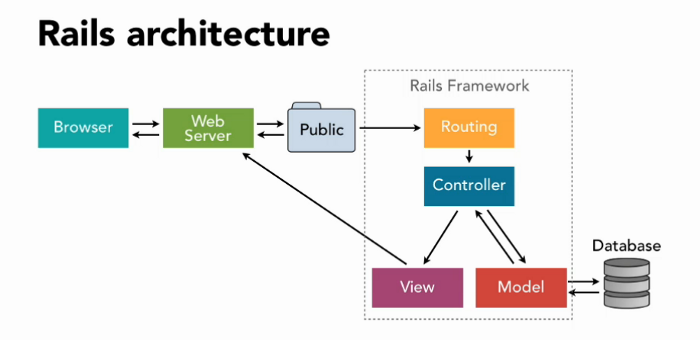
\includegraphics[width=.7\textwidth]{images/rails-arch.png}
  \end{center}

  \begin{block}{Information flows}
    \begin{itemize}
    \item User \(\to\) DB
    \item DB, public docs \(\to\) User
    \end{itemize}
    Annotate with BLP and Biba integrity levels. What security
    protection is needed?
  \end{block}

\end{frame}



\begin{frame}
  \frametitle{Classification in the Biba Model}

  \begin{block} {Quality Assurance Procedures}
    To elevate the integrity level of an information,
    \emph{sanitisation} procedures are needed
    \begin{itemize}
    \item Softwares, Networks:
      \begin{itemize}
      \item White box: Code review, static analysis
      \item Black box: Security coating to isolate the application
      \end{itemize}
    \item Data:
      \begin{itemize}
      \item Authenticity\&Audit
      \item End-to-end monitoring of process
      \end{itemize}
    \end{itemize}
  \end{block}


  \begin{block} {In practice}
    \begin{itemize}
    \item Aeronautics \& space: critical high-integrity systems
    \item Desire: integrate COTS to lower the cost of production
    \item Consequence: need for certification of these COTS
    \end{itemize}
  \end{block}


\end{frame}


\begin{frame}
  \frametitle{Logical Model}
  
  \begin{itemize}
  \item As in BLP, a lattice of Integrity levels
  \item Read/Write rules are reversed
  \end{itemize}

  \begin{block}{Pr{\'e}dicats}
    \begin{itemize}
    \item \p{ass}{x,l}: Subject $x$ has assurance level $l$
    \item \p{int}{x,l}: Object $x$ has integrity level $l$
    \item \p{read}{x,y}: Subject $x$ can read object $y$
    \item \p{wrt}{x,y}: Subject $x$ can write object $y$
    \item $l \preceq l'$: Assurance/Integrity level $l$ is lower than
      Assurance/Integrity level $l'$
    \end{itemize}
  \end{block}

  \pause

  \begin{block}{Access Control Rules}
    $$
    \begin{array}{rcl}
      \p{read}{x,y} & \gets& \p{ass}{x,l}, \p{int}{y,l'}, 
      \textcolor{red}{l \preceq l'}\\
      \p{wrt}{x,y} & \gets &\p{ass}{x,l}, \p{int}{y,l'}, 
      \textcolor{red}{l' \preceq l}\pause\\
      l \preceq l' & \gets & l \preceq l'', l'' \preceq l'\\
    \end{array}
    $$
  \end{block}

\end{frame}


\section{Model for Security}


\begin{frame}
  \frametitle{The show so far\(\ldots\)}

  \begin{block}{Assets}
    \begin{itemize}
    \item Information system is decomposed into segregated \emph{assets}
    \item Exceptions to this separation are to be controlled
    \end{itemize}
  \end{block}

  \vfill

  \begin{block}{Analysis, development}
    \begin{itemize}
    \item Analysis: difficulty to find a decomposition into assets
      that is manageable (small assets and few communications) and
      relevant
    \item Development: Programmers \textcolor{red}{must} keep in mind
      the place of the code they write in the global infrastructure
      to prepare for declassification and sanitisation procedures within the code
    \end{itemize}
  \end{block}

\end{frame}

\begin{frame}
  \frame{Graphical model}

  \begin{block}{Information system as a graph}
    \(G=(X,E,l_X,l_E)\):
    \begin{itemize}
    \item \(X\): set of assets (from inventory)
    \item \(E\): set of edges modelling the information flow
    \item \(l_X\) labelling of nodes (objects) with security and
      integrity levels
    \item \(L_E\): labelling of edges with all the subjects performing
      the data flow (can be network, specific softwares, humans)
    \end{itemize}
  \end{block}

  \vfill

  \begin{block}{Analysis}
    \begin{itemize}
    \item Assign default habilitation\&Assurance levels to subjects to
      ensure that all flows are permitted
    \item Compare these levels to desirable ones, and put in place
      classification/sanitsation procedures (coating or alteration) to
      elevate their levels to the desired ones
    \end{itemize}
  \end{block}
\end{frame}

\begin{frame}[fragile]
  \frametitle{Example: Web Server}
  
\begin{lstlisting}[language=Ruby]
class UsersController < ApplicationController
  before_action :set_user, only: [:show, :destroy,:update]
  before_filter :authenticate_user!, only: [:destroy,:update]
  after_action :verify_authorized
  ...
  def show
    authorize @user
  end
  ...
    def update_params
      params.require(:user).permit(policy(@user).permitted_attributes)
    end
end
\end{lstlisting}
\emph{authorize} and \emph{policy} global method managing access
control for the application 

\begin{block}{Good Practice: Fat Models, Skinny Controllers}
    \begin{itemize}
    \item Model: definition of the data stored in the DB, define the
      policy there (\lstinline[language=Ruby]|policy_attributes|)
    \item Controller (shown): methods handling the HTTP requests, just
      needs to check the policy, no definition of policy there
    \end{itemize}
  \end{block}
\end{frame}



\section{Availability and Proof}

\begin{frame}
  \frametitle{Beyond Existence, the Quantity}

  \vfill

  \begin{block}{Attack Examples}
    \begin{itemize}
    \item Denial of Service: flood a server with useless queries
    \item RansomWare: encrypt data on disk
    \end{itemize}
    Problem: lack/quality of access to the data 
  \end{block}

  \vfill

  \begin{block}{Availability}
    Ensuring timely and reliable access to and use of information
  \end{block}

  \vfill
  \end{frame}

  \begin{frame}
    \frametitle{Availability}

    \vfill

  \begin{block}{Relevance}
    \begin{itemize}
    \item Security mechanisms \emph{must} be available
    \item The usage of computer resources is one of the main goal of
      Information Security
    \item Often contradicts (and supercedes) NEAT's
      \emph{Non-bypassable} rule
    \end{itemize}
  \end{block}

  \vfill
  
  \begin{block}{Dilemna\&Resolution}
    \begin{itemize}
    \item Emphasis on availability: in case of unforeseen action, one
      must let the action be done (blacklisting rather than the more
      secure whitelisting)
    \item Safeguard: log the action for further processing \textit{if}
      it turned out to be malicious
    \end{itemize}
  \end{block}

  \vfill

\end{frame}

\begin{frame}
  \frametitle{Certification\&Accreditation (1/2)}

  \vfill

  \begin{block}{Certification}
    \begin{itemize}
    \item ``Proof'' that the system meets the security objectives
    \item Needs to cover all cases
    \end{itemize}
  \end{block}



  \vfill

  \begin{block}{Accreditation}
    ``Social choice'': 
    \begin{itemize}
    \item Given a certified system
    \item Approve it for certain usage
    \end{itemize}
    Constraints on a small drone are less stringents than on a
    civilian airframe
  \end{block}

\end{frame}

\begin{frame}
  \frametitle{Audit}

  \vfill

  \begin{block}{Definition}
    Independent review and examination of records and activities to
    assess the adequacy of system controls, to ensure compliance with
    established policies and operational procedures
  \end{block}

  \vfill

  \begin{block}{Notes}
    \begin{itemize}
    \item Based on logs describing the state of the system through time
    \item Rely on a sound association between processes\&humans
      \begin{itemize}
      \item \textcolor{red}{authentification} of the human responsible
        for a process
      \item \textcolor{red}{accountable} of an action to a process
        \begin{center}
          not just ``write access'', but what was written
        \end{center}
      \end{itemize}
    \end{itemize}
  \end{block}


  \vfill
\end{frame}

\begin{frame}
  \frametitle{Authentication\&Accountability}

  \vfill

  \begin{block}{Authentication}
    \begin{itemize}
    \item Processes \& humans are \emph{subjects}
    \item Access control can manage a bash terminal
    \item But to be relevant, must relate terminals to human users 
    \item Variant for data (code): data modifications must be related to users
    \end{itemize}
  \end{block}

  \vfill

  \begin{block}{Accountability}
    \begin{itemize}
    \item Having checked \(\neq\) having a proof
      \begin{itemize}
      \item You can check that users have read the license aggreement
      \item To have a proof, you need a MCQ and to store the results
        signed by the human
      \end{itemize}
    \item Relies ultimately on a proof of integrity of the security counter-measures
    \end{itemize}
  \end{block}

  \vfill

\end{frame}



\end{reveals}
\end{document}

